\documentclass[french]{beamer}
\usepackage{graphicx}
\usepackage{caption}

\usepackage[utf8]{inputenc}
\usepackage[T1]{fontenc}
\usepackage{lmodern}
\usepackage{amsmath, amssymb}

\usepackage{babel}


%CHOIX DU THEME et/ou DE SA COULEUR
% => essayer différents thèmes (en décommantant une des trois lignes suivantes)
%\usetheme{PaloAlto}
%\usetheme{Madrid}
%\usetheme{Copenhagen}
%\usetheme{CambridgeUS}

\usetheme{Hannover}

\useoutertheme[height=0pt,left]{sidebar}
\usecolortheme{beaver}
\setbeamercolor*{titlelike}{parent=structure}
\useinnertheme{circles}
\setbeamertemplate{frametitle}[default][right]



% => il est possible, pour un thème donné, de modifier seulement la couleur
%\usecolortheme{crane}
%\usecolortheme{seahorse}

%\useoutertheme[left]{sidebar}


%Pour le TITLEPAGE
\title{Analyse en Ondelettes}
\subtitle{Projet mathématiques-informatique}
\author[Rouyer, Gervais, Boulahia ]{ Chloé Rouyer, Pierre Gervais,  Souhaib Boulahia}
\date{\today}
\institute{Université Paris Diderot}


\begin{document}

\begin{frame}
	\titlepage
\end{frame}


\begin{frame}{Introduction}
	
	\begin{figure}[h]
		\centering
		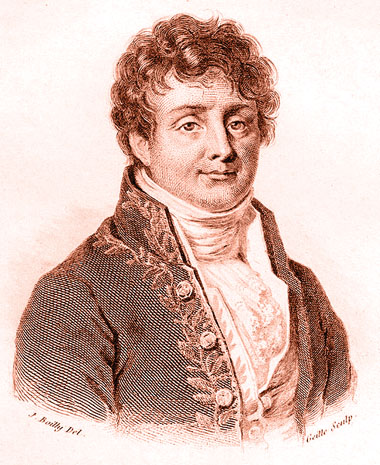
\includegraphics[width=100pt]{Fourier.jpg}
		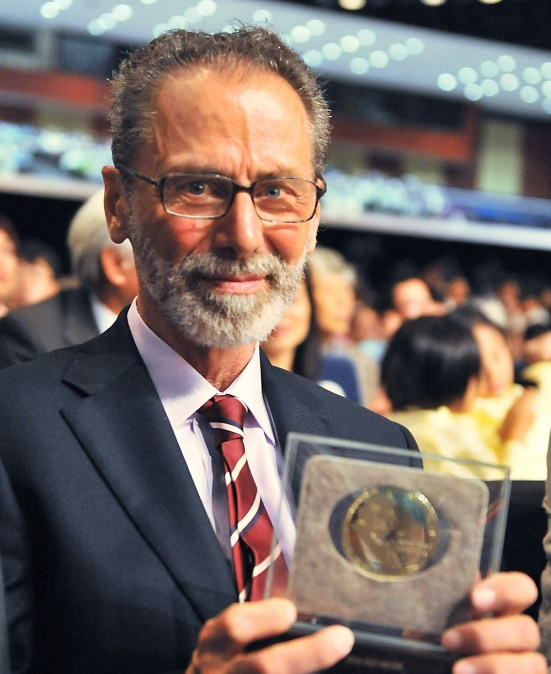
\includegraphics[width=100pt]{Meyer.jpg}
		\caption*{Joseph Fourier (1768 -1830) et Yves Meyer (1939- )}
	\end{figure}
	
\end{frame}

\begin{frame}{Sommaire}
	\tableofcontents
\end{frame}

\section{Outils}

\subsection{Analyse de Hilbert}
\begin{frame}{Problématique}
	
	\begin{itemize}
		\item<1-> Signaux : fonctions $\mathbb{R}^n \rightarrow \mathbb{R}^m$
		\item<2-> On veut généraliser les outils de la géométrie euclidienne
	\end{itemize}
		
\end{frame}

\begin{frame}{Problématique}
	\begin{itemize}
		\item<1-> $\ell^2$ et la famille $\{x_n = \delta(n - \cdot)\}_n$
		\item<2-> But : pouvoir écrire $$u = \sum_{n = 0}^{\infty} u_n x_n$$
	\end{itemize}
\end{frame}

\begin{frame}{Espace de Hilbert}
	Un \textit{espace de Hilbert} est la donnée
	\pause
	\begin{itemize}
		\item D'un espace vectoriel réel $E$ \pause
		\item D'un produit scalaire $\langle \cdot, \cdot \rangle$ défini sur $E$ \pause
		\item tel que $E$ soit complet pour la norme induite par ce produit scalaire
	\end{itemize}
\end{frame}

\begin{frame}{Espace de Hilbert séparable}
	$E$ est dit \textit{séparable} s'il existe $\mathbf{g} = \{g_n\}_{n \in \mathbb{N}}$ tel que $\overline{\mathbf{g}} = E$.
\end{frame}

\begin{frame}{Séparabilité et base hilbertienne}
	$E$ est séparable si et seulement s'il admet une base hilbertienne
	\pause
	où une \textit{base hilbertienne} est une famille orthonormée \textbf{totale}, c'est-à-dire une famille orthonormée $\mathcal{B}$ telle que $\text{Vect}(\mathcal{B})$ soit dense dans $E$.
\end{frame}

\begin{frame}{$E$ séparable $\Longleftrightarrow$ $E$ admet une base hilbertienne}
	$\mathbf{g} = \{g_n\}_{n \in \mathbb{N}} \subset E$ telle que $\overline{\mathbf{g}} = E$.\\
	\pause
	On orthonormalise par le procédé de Gramm-Schmidt $\mathbf{g}$ pour obtenir une famille $\mathbf{f}$ telle que $\text{Vect}(\mathbf{f}) = \text{Vect}(\mathbf{g})$ \pause $\supset \mathbf{g}$. \\
	\pause
	En passant à l'adhérence : $E = \overline{\mathbf{g}} \subset \overline{\text{Vect}(\mathbf{f})} \subset E$
\end{frame}

\subsection{Espaces de Lebesgue}

\begin{frame}
	Soit $(X, \mathcal{A}, \mu)$ un espace mesuré.\\
	\pause
	$$\mathcal{L}^p(X) = \left\{f ~: ~ X \to \mathbb{C} \text{ mesurable} ~ | ~ \int_X |f|^p d\mu < \infty \right\}$$
	\pause
	$\|f\|_p = \left(\displaystyle \int_X |f|^p d\mu \right)^{\frac{1}{p}}$
\end{frame}

\begin{frame}
		Soit la relation d'équivalence définie par $f \mathcal{R} g \Longleftrightarrow f \equiv g$ p.p.
		\pause
		$$L^p(X) = \mathcal{L}^p(X)/\mathcal{R}$$
		\pause
		$(L^p(X), \|\cdot\|_p)$ est alors normé ... \pause et complet !
\end{frame}




\section{Première approche : Analyse de Fourier}
\begin{frame}{Analyse de Fourier}
	\framesubtitle{Séries de Fourier}
	
	S'applique aux fonctions périodiques. 
	Dans $L^2(\mathbb{T})$
	\begin{itemize}
		\item<1-> Les $\{e^{-ikt}\}$ forment une base Hilbertienne
		\item<2-> $ \forall f \in L^2(\mathbb{T})$ on a $ S_N(f)= \sum_{k = -N}^N \langle f, e_k \rangle e_k = 
		\sum_{k = -N}^N c_k(f) e^{-ikt}  $ 
		\item<3-> Toute fonction de $L^2(\mathbb{T})$ se décompose dans la base des $\{e^{-ikt}\}$
		\item<4-> Et $ \lim\limits_{N \to \infty} \| S_N(f) - f \|_2  = f $ 
		
	\end{itemize}
	
\end{frame}

\begin{frame}{Preuve de $ \lim\limits_{N \to \infty} \| S_N(f) - f \|_2  = f $ }
	
	Soit $f \in L^2(\mathbb{T})$, soit $\varepsilon > 0$.\\
	Soit $f_0 \in L^2(\mathbb{T})$ une fonction continue telle que 
	$ \| f_0 - f \| < \varepsilon $\\
	\pause
	Soit $F_0$ tel que $f_0 = F_0(e^{it})$\\ 
	Il existe un polynôme $P$ tel que pour tout t, $\|f_0(t) - P(t)\| < \varepsilon$\\
	Ce qui permet de déduire que: \\
	\pause
	\begin{align*}
	\| S_N(f) -f \|_2 &\leqslant \|S_N(f) - S_N(P)\|_2 + \| S_N(P) - P \|_2 + \| f- P \|_2 \\
	&	\leqslant 2 \| f - P\|_2 + \| S_N(P) - P\|_2 \ \\
	& \leqslant 2 \| f - P\|_2  \\
	& \leqslant 2 \| f - f_0\|_2 + 2 \| f_0- P\|_2 \\
	& \leqslant 4 \varepsilon
	\end{align*}
	
	
\end{frame}






\section{Ondelettes et application}

\subsection{Analyse multi-résolution}

\begin{frame}{Analyse multi-résolution}
	Une \textit{analyse multi-résolution} de $L^2(\mathbb{R})$ est une famille de sous-espaces fermés $\{V_n\}_{n \in \mathbb{Z}} \subset L^2(\mathbb{R})$ telle que
	
	\pause
	$$\forall n \in \mathbb{Z}, ~ V_{n} \subset V_{n+1}$$

	\pause
	$$\forall n \in \mathbb{Z}, \forall f \in L^2(\mathbb{R}), ~ f \in V_n \Longleftrightarrow f (2 \, \cdot ) \in V_{n+1}$$
	
	\pause
	Il existe $\varphi$ telle que $\{\varphi_k = \varphi(\, \cdot + k)\}_{k \in \mathbb{Z}}$ forme une base orthonormée de $V_0$

	\pause
	$$\overline{\bigcup V} = L^2(\mathbb{R})$$
	
	\pause
	$$\bigcap V = \{0\}$$

	\pause			
	$\varphi$ est appelée \textit{fonction d'échelle}.
\end{frame}


\begin{frame}{L'espace de détails}
	L'espace $V_{n+1}$ est plus "fin" que $V_n$.\\
	\pause
	Soit $P_n ~ : ~ V_{n+1} \rightarrow V_n$ la projection orthogonale \pause $$W_n = \ker (P_n) \pause = V_{n+1}^\bot \cap V_n$$
	\pause
	On définit l'\textit{espace de détails} par
	$$V_{n+1} = W_n \oplus V_n$$\\
\end{frame}

\begin{frame}{L'espace de détails}
	\begin{align*}
		V_n &= V_{n-1} \oplus W_{n-1} \\
		&= V_{n-2} \oplus W_{n-2} \oplus W_{n-1} \\
		&\vdots \\
		&= \underbrace{\bigcap V}_{\{0\}} \oplus \left(\bigoplus_{k < n} W_k\right) \\
	\end{align*}

	\pause
	Et en faisant l'union pour tout $n \in \mathbb{Z}$ à droite et à gauche

	\pause
	$$\bigcup_{n \in \mathbb{Z}} V_n = \bigoplus_{n \in \mathbb{Z}} W_n \pause = V_0 \oplus \left(\bigoplus_{n \in \mathbb{N}} W_n\right)$$
\end{frame}

\begin{frame}{Les ondelettes}
	Il existe $\psi \in W_0$ tel que \\
	\pause
	\begin{itemize}
		\item $\{\psi(\cdot + k)\}_{k \in \mathbb{Z}}$ est une base orthonormée de $W_0$
		\pause
		\item $\displaystyle \int_{\mathbb{R}} \psi(t) dt = 0$ \\
	\end{itemize}
	\pause	
	
	La famille $\psi_{n, k}(t) = \sqrt{2^n}(2^n t - k)$ forme une famille orthonormée de $\displaystyle \bigoplus_{n \in \mathbb{Z}} W_n$\\
	\pause
	$\{\psi_{n, k}\}_{n, k \in \mathbb{Z}}$ est une base hilbertienne de $L^2(\mathbb{R})$ !
\end{frame}

\begin{frame}
	De $\displaystyle \bigcup_{n \in \mathbb{Z}} V_n = \bigoplus_{n \in \mathbb{Z}} W_n \pause = V_0 \oplus \left(\bigoplus_{n \in \mathbb{N}} W_n\right)$

	on déduit pour tout $f \in L^2(\mathbb{R})$
	
	$$f = \sum_{k \in \mathbb{Z}} \langle \varphi_k, f \rangle \varphi_k + \sum_{\substack{k \in \mathbb{Z} \\ n \in \mathbb{N}}} \langle \psi_{n, k}, f \rangle \psi_{n, k} = \sum_{\substack{k \in \mathbb{Z} \\ n \in \mathbb{Z}}} \langle \psi_{n, k}, f \rangle \psi_{n, k}$$
\end{frame}

\end{document}
















\begin{frame}
	Un \textbf<2,3>{texte} en gras. 
	\visible<3>{Un texte visible sur la 3\ieme{} couche}
\end{frame}

\begin{frame}{Titre (facultatif)} 
	\framesubtitle{Sous titre (facultatif aussi)}
	\begin{block}{Remarque}
		Un bloc
	\end{block}
	
	\begin{alertblock}{Proposition}
		Un bloc alerte
	\end{alertblock}
	
	\begin{exampleblock}<2>{Exemple}
		Un bloc exemple qui est visible sur la 2\ieme{} couche : $f(x)=2x$.
	\end{exampleblock}
\end{frame}

\section{Section 2}
\begin{frame}{La section 2 commence}
	\begin{itemize}
		\item<1-> On peut cliquer sur les titres de la barre de gauche pour naviguer dans les sections du pdf (essayez !).
		\item<2-> On peut changer le ``look'' du beamer, en changeant de thème. Retournez dans le fichier source et compilez avec les autres thèmes proposés (il existe énormément de thèmes; seuls trois sont proposés dans le source).
	\end{itemize}
	
\end{frame}